\documentclass[11pt]{report}
\usepackage{lscape}
\usepackage{bussproofs}
\usepackage{enumerate}
\usepackage{listings}
\usepackage{graphicx}
\usepackage{pdfpages}
\usepackage{titlesec}
\usepackage[hyphens]{url}
\usepackage{pgfgantt}
\usepackage{cite}
\usepackage{subfigure}
\usepackage{ textcomp }
\usepackage[a4paper, margin={1in,1in}]{geometry}
\graphicspath{ {../images/analysis/} }
\linespread{1.5}
\titleformat{\chapter}[block]{\normalfont\huge\bfseries}{\thechapter.}{1em}{\Huge}
\title{A Topological Interpretation of Place Cell Activity in the Rat Hippocampus : Data Analysis }
\linespread{1.5}
\date{2017-06-30}
\author{Hugh Osborne \\ sc16ho@leeds.ac.uk}
\begin{document}
\newpage
	\maketitle
\tableofcontents
\newpage
\chapter{Experiment Visualiser}
\section{Motivation}
In order to assess the feasibility of deriving a maze topology from experimental data, it was necessary to develop a simple application to visualise the location of the rat as it ran around a maze and the location at which spiking occurred. The expectation was, for each place cell, a distinct cluster of spiking activity would be visible as the rat passed through the corresponding place field. An assessment could then be made of the general size, shape, reliability and coverage of place fields for each experiment. Additionally, any noise or unexpected activity could be noted and perhaps explained using knowledge from the background research.

\section{Data}
Although it is assumed that only the spike timing data will be available when deriving the maze topology (as described in the Spatial Reconstruction Experiment), the Loren Frank experimental data and Pastalkova data \cite{pastalkova2008internally} contains a series of location points taken from the tracking of an LED attached to the rat as it moves around the maze. This can be used to create a computer animation of the rat. The position data represents interpolated positions at 30Hz and 39.06Hz for the respective experiment sets although the animation runs irrespective of real time. The important aspects of the animation are the position of the rat when a spike occurs and the order in which locations are visited. \\
The data is presented in an already processed manner in matlab MAT-files containing cell arrays of interpolated position data and time series of spikes. The spikes have been identified from the raw electrode potential difference signals and associated with individual cells. The Frank position data is partitioned in the following ways:\\
\begin{itemize}
\item By each rat subject, identified by the first three letters of its name
\item By the task the rat is performing (TrackA, TrackB or Sleep)
\item By the day and epoch (for example, Day 3 Epoch 4 is the third day of the experiment and the 4th activity performed by the rat on that day)
\end{itemize}

The spike data is further partitioned by tetrode number and unit number. There are on average, 17 units with some activity for each epoch. The Pastalkova position data is split into individual MAT-files for each activity (Figure 8 maze or platform exploration). There is no indication of day or epoch. The spike data is further partitioned by a cluster which represents the cell each spike is assumed to belong to.

\section{Extraction}
As the MAT-file is a proprietary binary format, the data must be extracted into a format which can be more easily parsed. To do this, two matlab scripts were written, tailored to the specific format of each experiment. Both scripts generate a `run.txt' file which lists time, x and y positions for each day and epoch (Pastalkova data day and epoch numbers are assigned values derived from the MAT-file filenames). Then, for each cluster or unit, a file is generated listing the times at which a spike is detected. If the MAT-file cell for this unit is empty or is below a certain threshold number of spikes, a file is not generated. This minimum spike parameter will be discussed along with others defined later in the process.\\
For ease of processing later, a file structure is built around these files as indicated in Figure \ref{fig:a}:

\begin{figure}[h!]
\begin{lstlisting}
<name>_<day>/
    process_input.txt
    <name>_<day>_<epoch>_activity/
        run.txt
        spikes/
        unit_<number>.txt
        smoothed/
        fields/
\end{lstlisting}
\caption{Visualiser Input File Structure}
\label{fig:a}
\end{figure}

process\_input.txt contains an index of all spike files with related file data for use later. The directories `smoothed' and `fields' likewise, are for use later.\\

\section{Visualisation}
An application was implemented to display a mouse icon which moves according to the position data in run.txt. It deposits a single sprite, a gaussian radial gradient, in the the rat's location in the event of a spike. The application was implemented in C++ utilising OpenGL GLUT due to its ease of setup, cross platform nature, extensive online support, and flexibility when compared to languages such as Java or Python.

\begin{figure}[h!]
\centering
  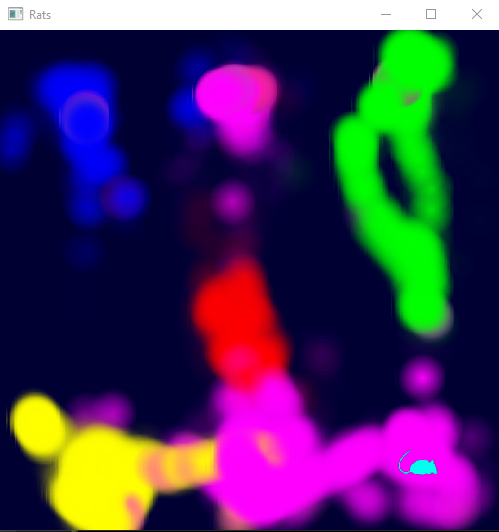
\includegraphics[width=0.3\textwidth]{placefields}
\caption{The visualiser application showing the mouse icon and five place fields derived from the spiking data of five different units}
\label{fig:b}
\end{figure}

The position data was normalised so that the extent of the maze corresponded to the size of the visualiser window. \\
In order to obtain more quantitative results beyond an animation, a single snapshot of all spikes at their corresponding locations was saved to a file and the screen was split into a grid. Each grid square was given a value corresponding to the number of spikes occurring while the rat's position was in the grid square divided by the total number of times the rat's position was recorded in that square. This `spike rate' value was normalised and displayed as a red colour in the image as well as recorded to a file. The `fields' directory generated in the extraction phase holds the image and the spike rate grid values are stored in a single file, placefields.txt, which contains the grids for all cells and epochs.

\begin{figure}[h!]
\centering
  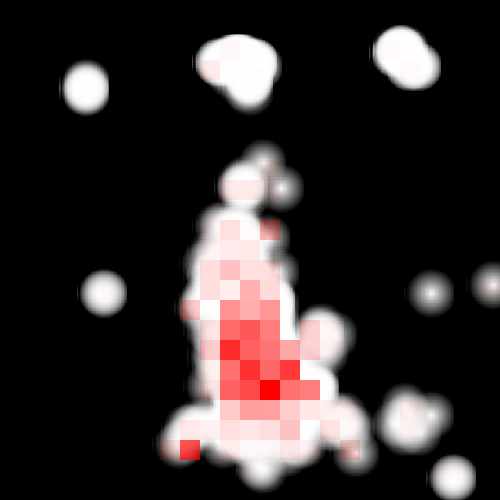
\includegraphics[width=0.3\textwidth]{grid}
\caption{A snapshot image of all spiking activity from a single unit file with the red “spike rate” grid overlay. The grid gives a good indication of where a place field is located and its extent by taking into account the number of spikes in a given area. This is in contrast to the white gaussian deposits which display dormant firing with the same intensity as place field firing.}
\label{fig:c}
\end{figure}

\newpage

\section{Smoothing}
It was expected that, in order to aid the estimation of topology, some smoothing would be required on the spiking data to minimise so called dormant spiking. That is, spikes which occur briefly at times when the rat is not inside its place field. To achieve this the time series of spikes from each unit file was split into discrete consecutive time bins and a hidden markov model was estimated with the following parameters:
 
\begin{itemize}
\item The probability of moving into a place field given the rat is currently outside.
\item The probability of moving out of a place field given the rat is currently inside.
\item The probability of observing a spike while inside a place field.
\item The probability of observing a spike while outside of a place field.
\end{itemize}
 
For each consecutive time bin, the probability that the rat is in each place field is estimated based on the observed number of spikes in that bin, the above parameters, and the probability estimated from the previous time bin. \\
This process is followed for each unit file. For each time bin, if the probability that the rat is outside of the place field is greater than inside the place field, the spikes in that bin are discarded. A new smoothed unit file is then generated and stored in the `smoothed' directory.

\section{Statistics Gathering}
The data files generated from the visualiser include the placefields.txt file, which contains the spike rate grid values, and the smoothed unit files, which contain the smoothed time series of spikes from each cell.\\
Python was used to further analyse this data due to its more functional nature and the simplicity of the pyplot library for plotting graphs.\\
Figure \ref{fig:d} summarises the number of cells showing spiking activity during a single epoch for three rats from the Frank experiments. In total there are eight rats whose data shall be used for testing and evaluation.

\begin{figure}[h!]
\caption{Place Cell Counts}
\centering
\begin{tabular}{|c|c|c|c|}
\hline
Name & Mean spiking units & max & min \\
\hline
Bond & 16.6 & 30 & 9 \\
\hline
Conley & 8.5 & 18 & 3 \\
\hline
Corriander & 14 & 20 & 7 \\
\hline
\end{tabular}
\label{fig:d}
\end{figure}
 
Once full data sets have been collated for figure 8, large platform and linear track experiments, their summaries will be added here.\\
 
As mentioned earlier, the spike rate grids give a good indication of where a place field is located and its extent by taking into account the number of spikes in a given area. Therefore, the placefields.txt files were used primarily for understanding the nature of the place fields in each experiment. Figure \ref{fig:e} shows the histogram of sizes of all place fields during both activities except sleeping (TrackA and TrackB) undertaken by the three rats across all days and epochs of the W maze experiments.
 
\begin{figure}[h!]
\caption{Histogram of Place Field Area (W track)}
\centering
  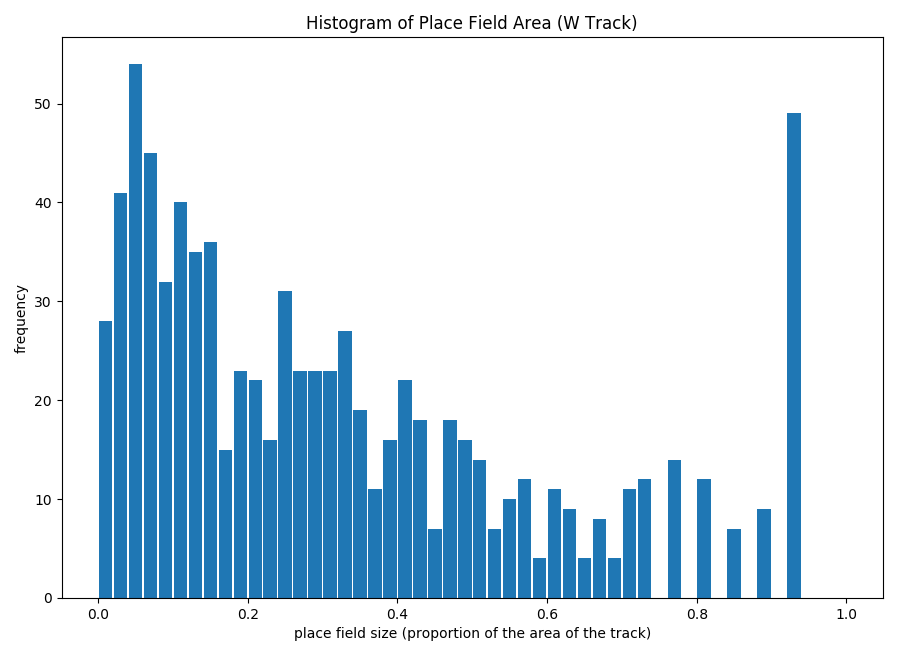
\includegraphics[width=0.6\textwidth]{wmaze_pf_size_histogram}
\label{fig:e}
\end{figure}
 
As a proportion of the size of each track, the place fields are generally quite large but with high variance. For the W maze, there is an outlying number of place fields covering almost the entire track. Without expert knowledge of the functioning of the electrodes and behaviour of cells in the hippocampus, it is difficult to say if these are indeed valid place fields derived from place cells or not. There are also a high proportion of place fields which take up almost no space at all on the track. Certain cells spike sporadically with no cohesive place field and these are recorded as such on the spike rate grid. It can be said that these are either not place cells or they code for a location which does not lie within the maze. These outlier cells will likely be a source of noise and it remains to be seen if it will affect the inference of topology.\\
 
For the W maze experiments, each rat was required to perform the alternation activity in two different mazes of the same shape many times over a number of days and/or epochs. If no remapping occurred between each of these activities, it would be useful to be able to take spike data from consecutive epochs to increase the confidence of the estimator. The correlation coefficient between two spike rate grids can provide a measure of how similar the place fields are for the same unit from two different epochs. In many cases, consecutive unit spike data is unavailable due to a negligible number of recorded spikes. This alone is an indication that remapping may be occurring between epochs, although shifts or failure in the tetrodes could also account for this. Figure \ref{fig:f} shows the average correlation coefficient between the first epoch and subsequent epochs for each available cell during Track A alternation activities for the three rats.

\begin{figure}[h!]
\caption{Average Correlation Coefficient between the First Epoch and Subsequent Epochs }
\centering
  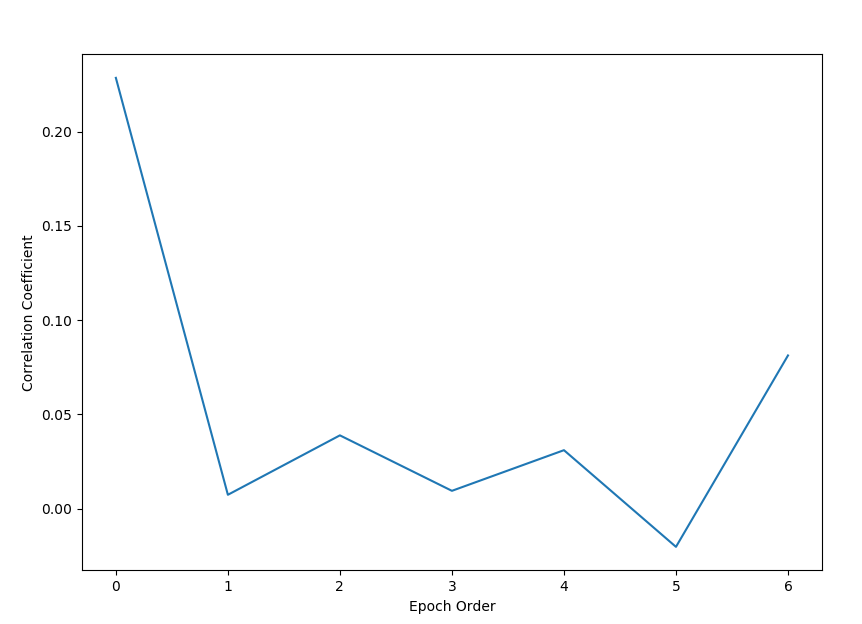
\includegraphics[width=0.6\textwidth]{correlation_by_epoch}
\label{fig:f}
\end{figure}
 
The correlation between the first and second epoch’s place field is generally higher, perhaps due to place fields remaining stable for the same track on the same day (for two of the three rats, the same activity was performed twice each day). After this, however, it seems there is no correlation. It is clear from this that the application will only be able to use spiking data from individual epochs to derive the topology. \\
 
Finally, one factor which would surely affect the ability of the application to estimate topology correctly is whether the place fields recorded in a single epoch cover the track fully. If it is the case that one arm of the W maze has no place fields or only large place fields which extend to the other arms as well, identifying this arm (and thus an arc from a junction node) would be impossible. 
To confirm acceptable coverage, the spike rate grids from each unit were summed and displayed as a heat map. For each epoch, two maps were generated, one with all place fields and one with only place fields smaller than 0.4 of the full size of the track. The stipulation of smaller place fields allow confirmation that full coverage is not only as a result of large place fields spanning the entire track. Figure \ref{fig:g} shows examples from different rats, mazes and epochs. The full set of results are available in the appendix. \\
 
\begin{figure}[h!]
\caption{Place Field Coverage : All Place Fields (left), Place Fields $<$ 0.4 (right)}
\centering
\subfigure{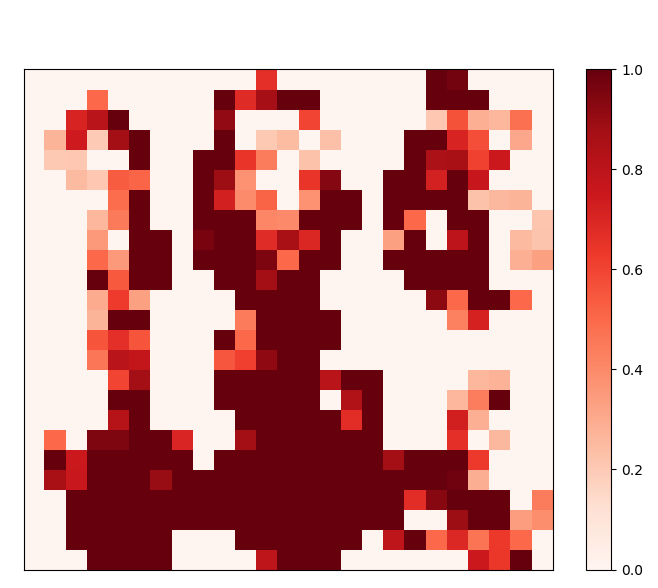
\includegraphics[width=0.2\textwidth]{coverage_bon_4_2_full}
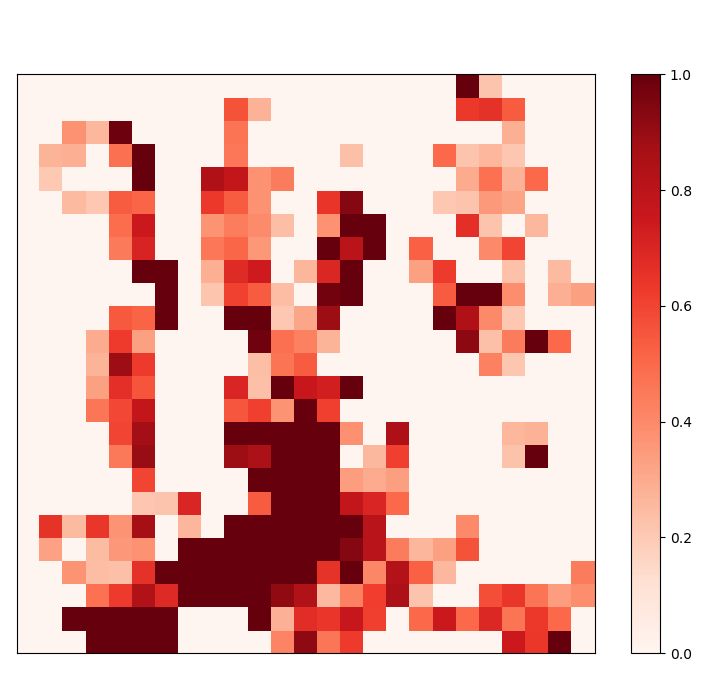
\includegraphics[width=0.2\textwidth]{coverage_bon_4_2_small}}

\subfigure{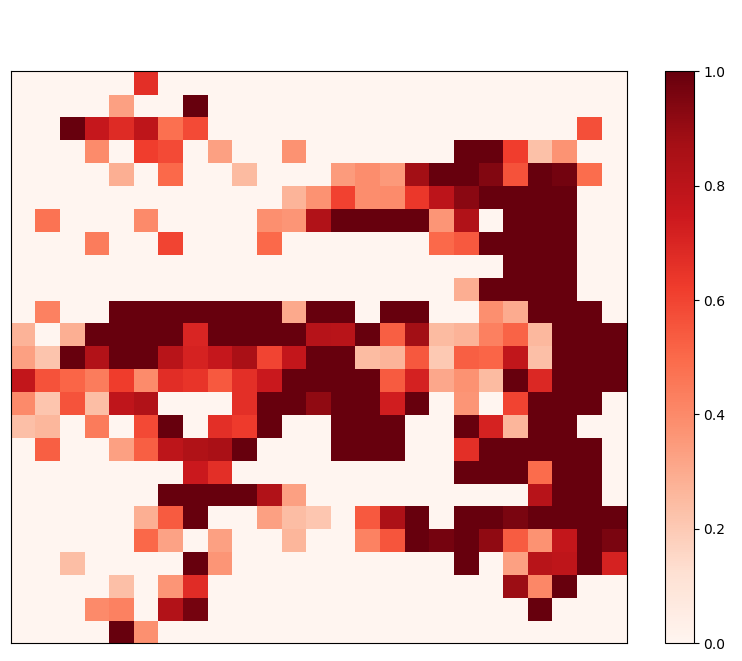
\includegraphics[width=0.2\textwidth]{coverage_bon_4_6_full}
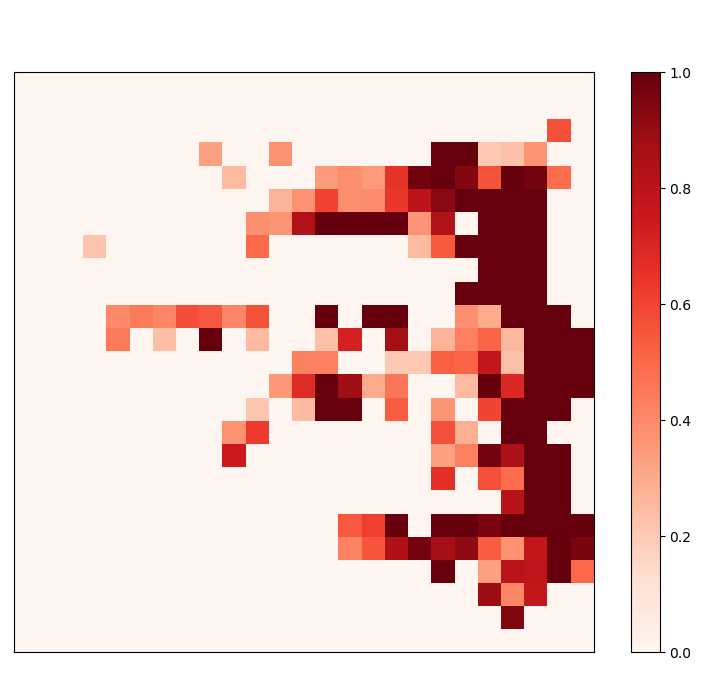
\includegraphics[width=0.2\textwidth]{coverage_bon_4_6_small}}

\subfigure{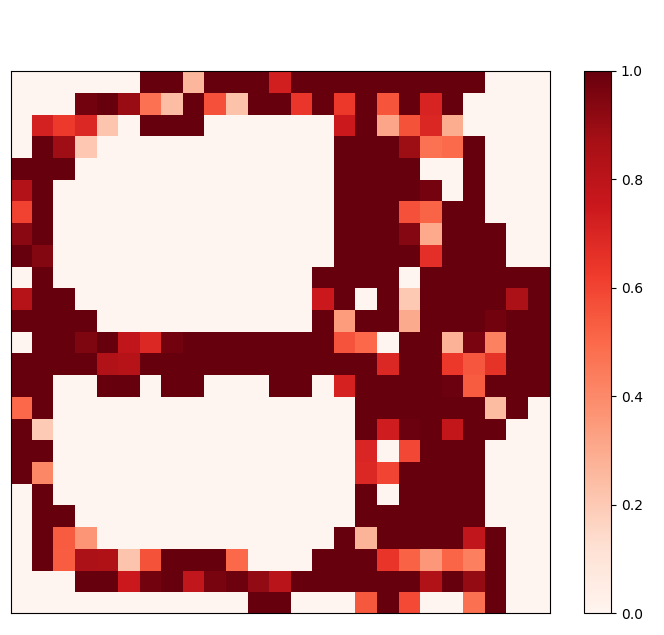
\includegraphics[width=0.2\textwidth]{coverage_maze_06_002_full}
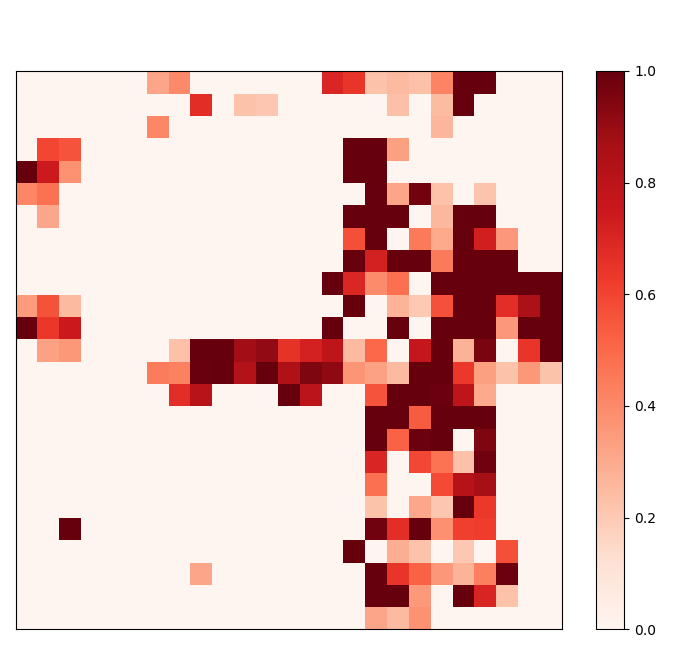
\includegraphics[width=0.2\textwidth]{coverage_maze_06_002_small}}

\label{fig:g}
\end{figure}

\chapter{Implementation and \\ Evaluation Plan}

\section{Adjacency Graph and Topology Estimation}
As discussed, the previous project estimated topology based on 200 simulated place cells with small (~1\% of the full track) place fields. The ordering and adjacency of place fields was defined as a set of RCC5 relations calculated from the simulated spike timings. From the RCC relations, the topology could then be deduced using a path finding technique. This was successful primarily due to the robustness of the RCC relations as would be expected from simulated data. Based on the findings above and the lack of success with experimental data in the previous project, a different appraoch is required to derive an adjacency graph in this case. Firstly, there are far fewer place cells and thus fewer place fields. This will reduce the confidence for an estimated topology as there will be less evidence to support it. Secondly, there is much higher variance in the size of the place fields, some spanning over half of the track and across junctions. This would cause difficulties in the path finding algorithm of the previous project which relies on the analysis of chains of small overlapping fields. One advantage to larger place fields, however, is that there is less chance of making false positives when identifying junctions as there will be few if any examples of a place field in a corridor having more than two adjacent fields. Finally, there is evidence of dormant firing and a number of examples of two or more distinct and separate place fields produced by a single cell. The RCC relations with these split place fields would surely cause issues for generating a robust model of the topology.\\
 
As there are much fewer partially overlapping place fields in the experimental data, it is difficult to use this characteristic as a measure of adjacency. Instead, the ordering of activity among the cells over time as the rat explores the maze can be used. That is, we can deduce that place field A is adjacent to place field B if place cell A fires and then place cell B fires immediately after. Due to the noisy nature of the data, however, it will be necessary to accumulate evidence of adjacency over the span of the time series to arrive at a confidence measure for a number of possible configurations. \\
As only the ordering of place cell activity is important, the spiking time series can be “compressed” to remove time bins which are empty. Consecutive duplicate time bins (with the same active cells) can be reduced to a single bin. \\

\paragraph{Intersecting Adjacency}
The intersecting adjacency algorithm iterates through each time bin in the compressed time series. The aim of this algorithm is to split the maze into distinct parts each representing a unique intersection of place fields. Adjacency can be deduced from the time series ordering of these intersections.

\begin{lstlisting}
For each time bin, t :
	Define the set of all active nodes in t, X.
	Define the set of all active nodes in t+1, Y.
	If no graph node representing X exists : 
		Create a node, node_X.
	If no graph node representing Y exists : 
		Create a node, node_Y.
	If no arc between node_X and node_Y exists : 
		Create an arc from node_X to node_Y with weight 1.
	Else : 
		Increment the weight for arc node_X to node_Y.
 
For each graph node :
	Normalise the weights of outgoing arcs.
	Discard arcs with weights lower than some threshold.
 
A junction node has at least three other adjacent nodes.
\end{lstlisting}

\paragraph{Non-Intersecting Adjacency}
The non-intersecting adjacency algorithm again iterates through each time bin of the compressed time series. This algorithm aims to find non intersecting place fields and deduce their adjacency ignoring other intermediate overlapping fields.\\

\begin{lstlisting}
For each unit, x :
    For each time bin, t :
        If x is active in t and not active in t+1 :
            Starting at t+1, find the next time bin such that 
               x is not active and 
               there exists an active unit, y which was not active in t.
           If there is more than one candidate for y :
               Choose y represented by the graph node with highest weight.
           If no graph node representing x exists : 
               Create a node, node_x.
           If no graph node representing y exists : 
               Create a node, node_y.
           If no arc between node_x and node_y exists : 
               Create an arc from node_x to node_y with weight 1.
           Else : 
               Increment the weight for arc node_x to node_y.
	
    Normalise the weights of outgoing arcs for node_x.
    Discard arcs with weights lower than some threshold.
 
    Node_x is a junction node if it has at least three other adjacent nodes.		
\end{lstlisting}

For both algorithms it should be possible to identify the end of corridors by graph nodes with degree one. Questions remain about how to deal with particularly large place fields which subsume one or more other fields. This is a similar problem to cells with multiple place fields. \\
Further investigation will be required to confirm that mazes with loops (as with the figure 8 maze) are correctly described.\\

\section{Parameters}
During both the pre-processing of the experimental data and in the algorithms themselves, the following parameters have been defined which will affect the performance of topology estimation:\\
\begin{itemize}
\item A Minimum number of spikes recorded from a single unit
\item The probability parameters used in the HMM smoothing step
\item The weight threshold for arcs in the adjacency graph
\end{itemize}
 
Once the full solution has been implemented, it will be necessary to perform a sensitivity analysis on these parameters to quantify the robustness of the solution to other data sets. In particular, to what extent do changing these parameters alter the Precision, Recall and ROC (Receiver Operator Characteristic) performance metrics. During testing, it may become apparent that additional constraints on the data need to be made and these should be included in the analysis.\\

\section{Evaluation}
If the spatial reconstruction thought experiment is sound, estimating the topology from the spiking activity amounts to a classification task and so can be evaluated as such. Experimental cell data is available for W shaped and figure 8 mazes as well as linear tunnels and large platforms. Figure \ref{fig:h} lists the various topological characteristics which may be deducible from the adjacency graph for each configuration.

\begin{figure}[h!]
\caption{Configuration Characteristics}
\centering
\begin{tabular}{|c|c|c|c|}
\hline
Configuration & Junctions & Loops & `Dead-ends' \\
\hline
W maze & 1 (degree 3) & 0 & 3 \\
\hline
Figure 8 & 2 (degree 3) or possibly 1 (degree 4) & 2 & 0 \\
\hline
Linear & 0 & 0 & 2 \\
\hline
Platform & Many & Many & 0 \\
\hline
\end{tabular}
\label{fig:h}
\end{figure}

It is expected that the idealised adjacency graph derived from a platform or arena will have many nodes with high degree (representing fields in the centre of the platform), nodes with lower degree (fields around the edge and in the corners), many loops and no dead ends. However, arcs belonging to nodes with high degree may be discarded (their normalised weights will be low due to the high degree) and so the graph may end up looking like a large ring. From a topological perspective, this is perhaps the `desired' result. \\
 
For each topological characteristic, a confusion matrix can be produced based on the output estimate and the known source of the input data. Deriving precision-recall graphs from these will be useful for comparing performance of the “intersecting” and “non intersecting” algorithms. Due to the relatively small number of total available data sets and the difference in data sets available for each configuration, there is a potential for bias in the precision and recall metrics. An increasingly popular alternative is the Receiver Operator Characteristic (ROC) which takes into account the difference in available positive and negative samples. The ROC Area gives a performance scale from 0.5 which indicates random choice, to 1 which indicates perfect estimation. When performing the sensitivity analysis, it will be useful to track a single performance value as each parameter is adjusted. The ROC Area will be a good choice for this. Alternatively, a cost value could be applied to false positives and false negatives (leaving 0 cost for true positives and negatives). The minimum total cost could be calculated for a given set of results and plotted against the change in each parameter. The challenge would be to justify a cost ratio between FPs and FNs.\\

\newpage
\medskip
\bibliographystyle{plain}
\bibliography{coursework1}

\appendix

\end{document}